\documentclass{standalone}
\usepackage{tikz-network}

\begin{document}
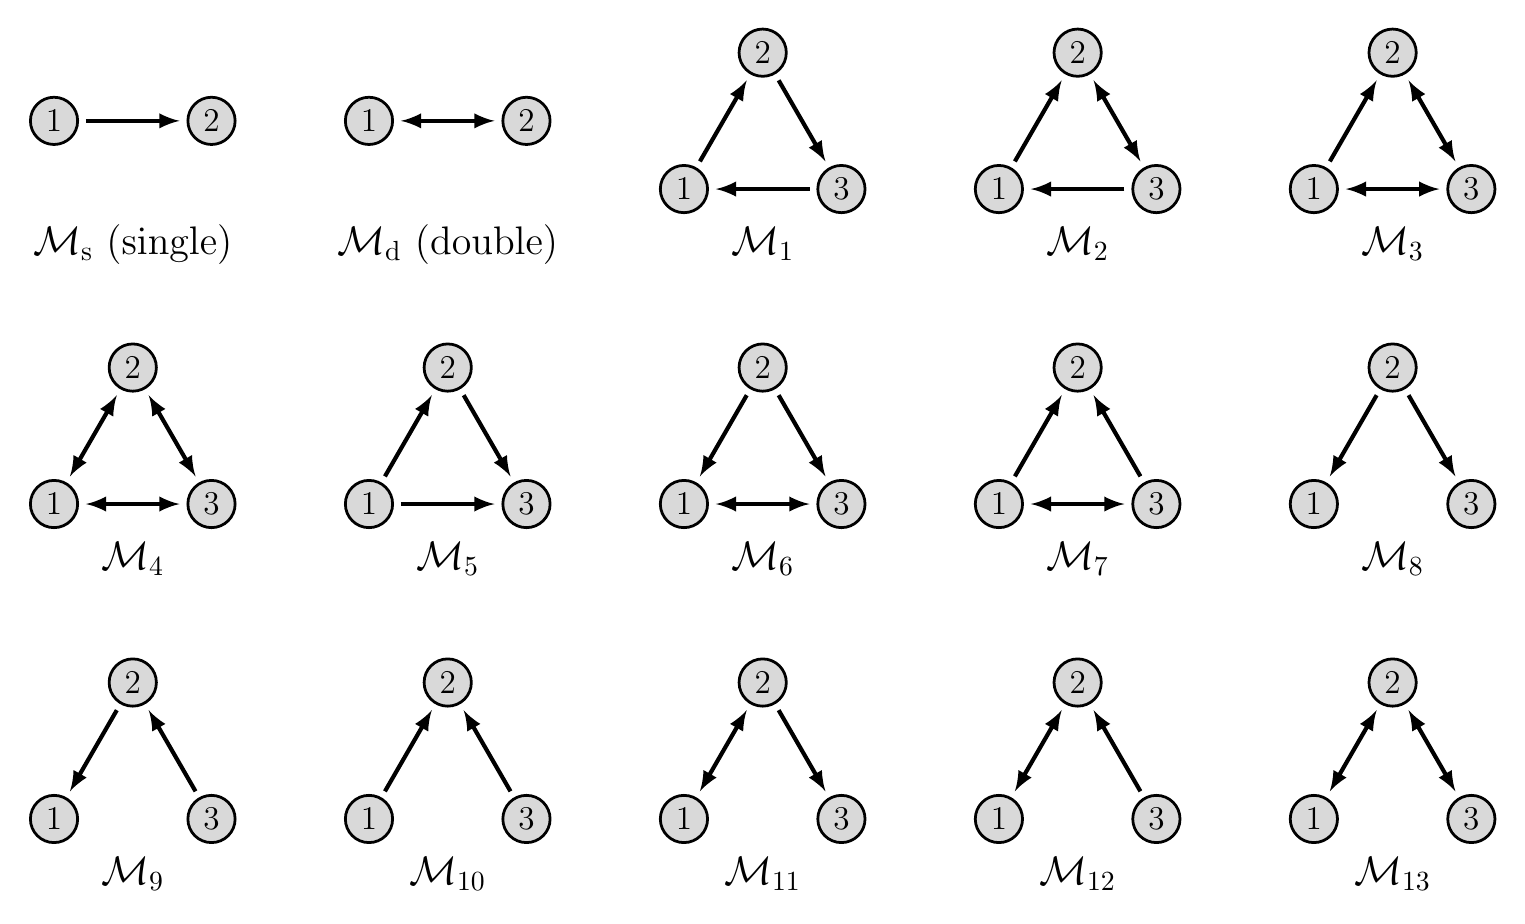
\begin{tikzpicture}

\SetVertexStyle[LineWidth=1, FillColor=black!15!white, LineColor=black, OuterSep=3, TextFont=\large]
\SetEdgeStyle[Color=black]
\SetTextStyle[TextFont=\Large]

% Row 1

\Vertex[x=0,y=0.866,label=1]{Me1_1}
\Vertex[x=2,y=0.866,label=2]{Me1_2}
\Edge[Direct](Me1_1)(Me1_2)
\Text[x=1,y=-0.7]{$\mathcal{M}_\mathrm{s}$ (single)}

\Vertex[x=4,y=0.866,label=1]{Me2_1}
\Vertex[x=6,y=0.866,label=2]{Me2_2}
\Edge[Direct,style=latex-latex](Me2_1)(Me2_2)
\Text[x=5,y=-0.7]{$\mathcal{M}_\mathrm{d}$ (double)}
 
\Vertex[x=8,label=1]{M1_1}
\Vertex[x=9,y=1.732,label=2]{M1_2}
\Vertex[x=10,label=3]{M1_3}
\Edge[Direct](M1_1)(M1_2)
\Edge[Direct](M1_2)(M1_3)
\Edge[Direct](M1_3)(M1_1)
\Text[x=9,y=-0.7]{$\mathcal{M}_1$}

\Vertex[x=12,label=1]{M2_1}
\Vertex[x=13,y=1.732,label=2]{M2_2}
\Vertex[x=14,label=3]{M2_3}
\Edge[Direct](M2_1)(M2_2)
\Edge[Direct,style=latex-latex](M2_2)(M2_3)
\Edge[Direct](M2_3)(M2_1)
\Text[x=13,y=-0.7]{$\mathcal{M}_2$}

\Vertex[x=16,label=1]{M3_1}
\Vertex[x=17,y=1.732,label=2]{M3_2}
\Vertex[x=18,label=3]{M3_3}
\Edge[Direct](M3_1)(M3_2)
\Edge[Direct,style=latex-latex](M3_2)(M3_3)
\Edge[Direct,style=latex-latex](M3_3)(M3_1)
\Text[x=17,y=-0.7]{$\mathcal{M}_3$}

% Row 2

\Vertex[x=0,y=-4,label=1]{M4_1}
\Vertex[x=1,y=-2.267,label=2]{M4_2}
\Vertex[x=2,y=-4,label=3]{M4_3}
\Edge[Direct,style=latex-latex](M4_1)(M4_2)
\Edge[Direct,style=latex-latex](M4_2)(M4_3)
\Edge[Direct,style=latex-latex](M4_3)(M4_1)
\Text[x=1,y=-4.7]{$\mathcal{M}_4$}

\Vertex[x=4,y=-4,label=1]{M5_1}
\Vertex[x=5,y=-2.267,label=2]{M5_2}
\Vertex[x=6,y=-4,label=3]{M5_3}
\Edge[Direct](M5_1)(M5_2)
\Edge[Direct](M5_1)(M5_3)
\Edge[Direct](M5_2)(M5_3)
\Text[x=5,y=-4.7]{$\mathcal{M}_5$}

\Vertex[x=8,y=-4,label=1]{M6_1}
\Vertex[x=9,y=-2.267,label=2]{M6_2}
\Vertex[x=10,y=-4,label=3]{M6_3}
\Edge[Direct](M6_2)(M6_1)
\Edge[Direct](M6_2)(M6_3)
\Edge[Direct,style=latex-latex](M6_1)(M6_3)
\Text[x=9,y=-4.7]{$\mathcal{M}_6$}

\Vertex[x=12,y=-4,label=1]{M7_1}
\Vertex[x=13,y=-2.267,label=2]{M7_2}
\Vertex[x=14,y=-4,label=3]{M7_3}
\Edge[Direct](M7_1)(M7_2)
\Edge[Direct](M7_3)(M7_2)
\Edge[Direct,style=latex-latex](M7_1)(M7_3)
\Text[x=13,y=-4.7]{$\mathcal{M}_7$}

\Vertex[x=16,y=-4,label=1]{M8_1}
\Vertex[x=17,y=-2.267,label=2]{M8_2}
\Vertex[x=18,y=-4,label=3]{M8_3}
\Edge[Direct](M8_2)(M8_1)
\Edge[Direct](M8_2)(M8_3)
\Text[x=17,y=-4.7]{$\mathcal{M}_8$}

% Row 3

\Vertex[x=0,y=-8,label=1]{M9_1}
\Vertex[x=1,y=-6.267,label=2]{M9_2}
\Vertex[x=2,y=-8,label=3]{M9_3}
\Edge[Direct](M9_2)(M9_1)
\Edge[Direct](M9_3)(M9_2)
\Text[x=1,y=-8.7]{$\mathcal{M}_9$}

\Vertex[x=4,y=-8,label=1]{M10_1}
\Vertex[x=5,y=-6.267,label=2]{M10_2}
\Vertex[x=6,y=-8,label=3]{M10_3}
\Edge[Direct](M10_1)(M10_2)
\Edge[Direct](M10_3)(M10_2)
\Text[x=5,y=-8.7]{$\mathcal{M}_{10}$}

\Vertex[x=8,y=-8,label=1]{M11_1}
\Vertex[x=9,y=-6.267,label=2]{M11_2}
\Vertex[x=10,y=-8,label=3]{M11_3}
\Edge[Direct,style=latex-latex](M11_1)(M11_2)
\Edge[Direct](M11_2)(M11_3)
\Text[x=9,y=-8.7]{$\mathcal{M}_{11}$}

\Vertex[x=12,y=-8,label=1]{M12_1}
\Vertex[x=13,y=-6.267,label=2]{M12_2}
\Vertex[x=14,y=-8,label=3]{M12_3}
\Edge[Direct,style=latex-latex](M12_1)(M12_2)
\Edge[Direct](M12_3)(M12_2)
\Text[x=13,y=-8.7]{$\mathcal{M}_{12}$}

\Vertex[x=16,y=-8,label=1]{M13_1}
\Vertex[x=17,y=-6.267,label=2]{M13_2}
\Vertex[x=18,y=-8,label=3]{M13_3}
\Edge[Direct,style=latex-latex](M13_1)(M13_2)
\Edge[Direct,style=latex-latex](M13_3)(M13_2)
\Text[x=17,y=-8.7]{$\mathcal{M}_{13}$}

\end{tikzpicture}
\end{document}